\chapter{Leer los datos y aumentarlos}
\label{cap:datos}

\begin{enpocas}
Cómo se cargan las imágenes y sus etiquetas, cómo se llevan a $640\times640$ sin
deformarlas (letterbox) y qué aumentos se aplican para que 5\,400 imágenes
alcancen. Archivo: \cod{red_fuego/datos.py}.
\end{enpocas}

\section{De archivo a tensor}

\paso{17} \textbf{Escribir \cod{DatasetYolo}.}
Un \cod{Dataset} de PyTorch solo necesita dos métodos: \cod{__len__} (cuántas
muestras hay) y \cod{__getitem__(i)} (dame la muestra $i$). El
\cod{DataLoader} los usa para armar lotes en paralelo con varios procesos
(\cod{num_workers=8}).

Cada muestra devuelve la imagen como tensor \cod{uint8} $(3, 640, 640)$ en RGB y
una tabla de etiquetas $(n, 5)$ con \cod{clase, cx, cy, w, h} normalizados.
La función \cod{juntar} une un lote y agrega a cada etiqueta el índice de su
imagen, porque cada imagen tiene un número distinto de objetos.

\section{Letterbox: cambiar de tamaño sin deformar}

La cámara da $640\times480$ y la red quiere $640\times640$. Estirar la imagen
deformaría las llamas. \textbf{Letterbox} la escala para que el lado mayor mida
640 y rellena el resto con gris (valor 114). Para esta cámara: escala $r = 1$ y
80 píxeles de gris arriba y abajo. Al inferir hay que deshacerlo:
$x_{\text{orig}} = (x - d_x)/r$, $y_{\text{orig}} = (y - d_y)/r$.

\section{Aumentos de datos}

El simulador tiene la luz siempre igual, los mismos árboles y el mismo fuego. Si
la red solo ve eso, aprende detalles que no se repiten en el mundo real (el
\emph{sobreajuste}). Los aumentos crean variantes nuevas en cada época:

\begin{description}
  \item[Mosaico] Cuatro imágenes en un lienzo de $1280\times1280$, alrededor de un
        centro al azar; luego se recorta a $640\times640$. La red ve objetos
        partidos, a varias escalas y con contextos mezclados. Es el aumento que más
        ayuda a YOLO.
  \item[Afín] Escala al azar entre 0.5 y 1.5 y traslación de $\pm10$\,\%. Simula
        volar más alto o más bajo. Las cajas se transforman con la misma matriz y se
        descartan las que quedan casi fuera (menos de 2 píxeles o menos del 10\,\%
        de su área).
  \item[HSV] Tono $\pm1.5$\,\%, saturación $\pm50$\,\% y brillo $\pm40$\,\% con
        tablas de búsqueda (rápido). Simula otra hora del día u otra cámara.
  \item[Espejo] Horizontal con probabilidad 0.5.
\end{description}

\paso{18} \textbf{Ver los aumentos antes de entrenar.}
Este es el paso más importante del capítulo: si las cajas no coinciden con el
fuego después de aumentar, la red aprende basura y el error no aparece en ningún
lado.

\begin{lstlisting}[style=py]
from cuadrirotor_sim.red_fuego.datos import DatasetYolo
ds = DatasetYolo('.../data.yaml', 'train', 640, aumentar=True)
img, e = ds[3000]                     # dibuja e sobre img y guárdala
\end{lstlisting}

\begin{figure}[H]
\centering
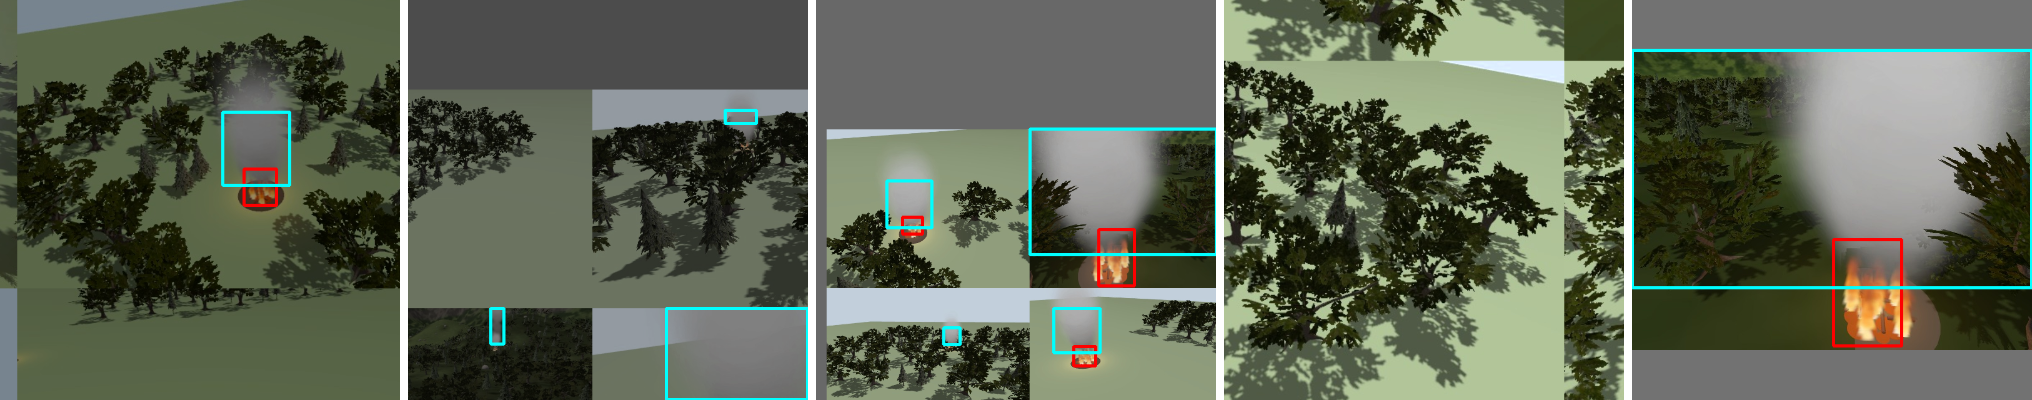
\includegraphics[width=\textwidth]{aumentos.png}
\caption{Cuatro muestras aumentadas (mosaico + afín + HSV + espejo) y una de
validación sin aumentar (derecha). Rojo: fuego. Cian: humo.}
\label{fig:aumentos}
\end{figure}

\begin{resultado}
Cada caja roja encierra llamas y cada caja cian una columna de humo, incluso en
los pedazos del mosaico. Las franjas grises son el relleno.
\end{resultado}

\begin{consejo}
En las últimas 10 épocas se apaga el mosaico (\cod{--sin-mosaico 10}). Así la
red termina viendo imágenes como las que verá en vuelo. Como los procesos del
\cod{DataLoader} guardan su propia copia del dataset, al cambiar
\cod{ds.mosaico} hay que crear un \cod{DataLoader} nuevo.
\end{consejo}

\begin{leccion}
Las etiquetas de las imágenes sin fuego son archivos vacíos y
\cod{np.loadtxt} da un aviso por cada uno (más de mil líneas en la terminal). Se
revisa el tamaño del archivo antes de leerlo:
\begin{lstlisting}[style=py]
    if not os.path.exists(p) or os.path.getsize(p) == 0:   # imagen sin fuego ni humo
        return np.zeros((0, 5), np.float32)
\end{lstlisting}
\end{leccion}
